%! TEX root = BusinessAnalysis.tex
\documentclass[11pt,a4paper]{article}

\usepackage[utf8]{inputenc}
\usepackage[margin=1in]{geometry}
\usepackage{xcolor}
\usepackage{hyperref}
\usepackage{longtable}
\usepackage{booktabs}
\usepackage{array}
\usepackage{graphicx}
\usepackage{calc}
\usepackage{listings}

\lstdefinelanguage{json}{
    basicstyle=\small\ttfamily,
    numbers=left,
    numberstyle=\tiny\color{gray},
    stepnumber=1,
    numbersep=8pt,
    showstringspaces=false,
    breaklines=true,
    frame=lines,
    backgroundcolor=\color{black!3},
    stringstyle=\color{red!70!black},
    keywordstyle=\color{blue!80!black}
}

\title{\textbf{Business Analysis\\Multi-sig}}
\author{\LARGE{Hazaparu Sorin-Daniel}}
\date{\today}

\begin{document}

\maketitle
\newpage

\section{Executive Summary \& Vision}

\textbf{Product name:} Multi-sig \\
\textbf{Domain:} Banking / Payments / Secure signatures \\
\textbf{Problem Statement:} Companies need multiple signatures for
approving and distributing salaries, invoices, Liquidity Sweeps etc. \\
\textbf{Target Audience:} Companies, Executives and employees \\
\textbf{Value Proposition:} Reduces wait time for signatures and
eliminates bookkeeping errors

\section{Scope Definition}

\textbf{A. In-Scope:}

\begin{itemize}
\item
  Role-Based Access Control, Signatures and Uploads
\item
  Web interface for users to sign
\item
  Loging of every action
\item
  Locking file between submission and delivery
\item
  No self-approving of documents
\item
  Dynamic Threshold, based on the sum of money, the amount will require
  different approvals
\item
  Veto for payments
\end{itemize} 
\textbf{B. Out-of-Scope:}

\begin{itemize}
\item
  Serverless option for big companies
\item
  MFA
\item
  Hardware Keys
\item
  VPN / ZTNA
\item
  Infrastructure for different/customizable file types with custom APIs
  and hooks, but a system to add different files will be in place
\item
  Any form of external API (Like AWS S3)
\end{itemize}
\newpage
\section{Users Personas}

\begin{longtable}[]{@{}
  >{\centering\arraybackslash}p{(\linewidth - 6\tabcolsep) * \real{0.2499}}
  >{\centering\arraybackslash}p{(\linewidth - 6\tabcolsep) * \real{0.2499}}
  >{\centering\arraybackslash}p{(\linewidth - 6\tabcolsep) * \real{0.2501}}
  >{\centering\arraybackslash}p{(\linewidth - 6\tabcolsep) * \real{0.2501}}@{}}
\toprule\noalign{}
\begin{minipage}[b]{\linewidth}\raggedright
Persona Name
\end{minipage} & \begin{minipage}[b]{\linewidth}\raggedright
Role / Description
\end{minipage} & \begin{minipage}[b]{\linewidth}\raggedright
Primary Goals
\end{minipage} & \begin{minipage}[b]{\linewidth}\raggedright
Key Pain Points
\end{minipage} \\
\midrule\noalign{}
\endhead
\bottomrule\noalign{}
\endlastfoot
Jhon (High ranking employee) & Employee of a given company & Signing and
approving different payment numbers & Handling multiple excels sent via
email and signing over them can introduce a lot of friction \\
Robbert (Regular Employee) & Employee of a given company & Regular work
& Waiting for salary or any work related payments to be approved without
knowing why or who is responsible for the delay can lead to
impatience \\
Andrew (CEO) & CEO of a given company & Meetings and approvals &
Reviewing every payment can be overwhelming \\
Peter (CFO) & CFO of a given company & Meetings and approvals & Checking
every payment from different excels sent via email can take substantial
time \\
\end{longtable}

\textbf{\hfill\break
}

\section{Requirements Specification}

\subsection{Functional Requirements}

\textbf{FR-01} Authorization and roles: The system must enforce roles
and permissions for `System Admin', `CEO', `CFO', `Employee', `Manager',
`Board Director', `Accountant' directed by this table:

\begin{longtable}[]{@{}
  >{\centering\arraybackslash}p{(\linewidth - 8\tabcolsep) * \real{0.2394}}
  >{\centering\arraybackslash}p{(\linewidth - 8\tabcolsep) * \real{0.1984}}
  >{\centering\arraybackslash}p{(\linewidth - 8\tabcolsep) * \real{0.1941}}
  >{\centering\arraybackslash}p{(\linewidth - 8\tabcolsep) * \real{0.1971}}
  >{\centering\arraybackslash}p{(\linewidth - 8\tabcolsep) * \real{0.1710}}@{}}
\toprule\noalign{}
\begin{minipage}[b]{\linewidth}\centering
Role
\end{minipage} & \begin{minipage}[b]{\linewidth}\centering
Can request business expense
\end{minipage} & \begin{minipage}[b]{\linewidth}\centering
Can upload salary or payroll invoice
\end{minipage} & \begin{minipage}[b]{\linewidth}\centering
Can approve
\end{minipage} & \begin{minipage}[b]{\linewidth}\centering
Can Veto
\end{minipage} \\
\midrule\noalign{}
\endhead
\bottomrule\noalign{}
\endlastfoot
System Admin & Yes & No & No & No \\
Employee & Yes & No & No & No \\
Manager & Yes & Yes & Yes & No \\
Board Director/CEO/CFO & Yes & Yes & Yes & Yes \\
Accountant & Yes & Yes & No & No \\
\end{longtable}
\noindent\textbf{FR-02} Signing process: The requester must not be allowed to
approve or sign its own request.
\newpage
\noindent\textbf{FR-03} Interface: The system must provide a web interface that
will display the current requests. If a user has permission to upload or
request, an interface to upload must appear. Each user should be able to
see its Personal Requests, if present they should be able to see who has
yet to sign, or if denied, they should be able to see any
comments/reasons, if any were provided. Additionally, each user should
also see the following based on the role:

\begin{itemize}
\item
  Accountant: Its own payroll invoice.
\item
  Manager: Requests from users within their reporting hierarchy.
\item
  Board Director/CEO/CFO: All requests.
\item
  System Admin: Metadata, Option to manage Roles and Audit Logs.
\end{itemize}

\noindent\textbf{FR-04} Webpage Security: The system must enforce strict Username
and Password login. \\
\textbf{FR-05} System Admin: The system admin must be able to pause all
transactions. The transactions shall not be canceled or denied, instead
no action can be taken. A notification should appear on the webpage
informing other users about the current state. \\
\textbf{FR-06} Files: If the user uploads salary or invoice file the
structure must be verified at upload, with strong feedback on
malformation (Row, Col and Reason), be CSV and have the structure:

\begin{longtable}[]{@{}
  >{\raggedright\arraybackslash}p{(\linewidth - 8\tabcolsep) * \real{0.2000}}
  >{\raggedright\arraybackslash}p{(\linewidth - 8\tabcolsep) * \real{0.2000}}
  >{\raggedright\arraybackslash}p{(\linewidth - 8\tabcolsep) * \real{0.2000}}
  >{\raggedright\arraybackslash}p{(\linewidth - 8\tabcolsep) * \real{0.2000}}
  >{\raggedright\arraybackslash}p{(\linewidth - 8\tabcolsep) * \real{0.2000}}@{}}
\toprule\noalign{}
\begin{minipage}[b]{\linewidth}\raggedright
From
\end{minipage} & \begin{minipage}[b]{\linewidth}\raggedright
To
\end{minipage} & \begin{minipage}[b]{\linewidth}\raggedright
Reason
\end{minipage} & \begin{minipage}[b]{\linewidth}\raggedright
Amount
\end{minipage} & \begin{minipage}[b]{\linewidth}\raggedright
Currency
\end{minipage} \\
\midrule\noalign{}
\endhead
\end{longtable}
\noindent\textbf{FR-07} Approval and Denial: Any request should be approved by a
simple click and confirmation. On denial the denier can leave a
comment/message/reason on why it was denied.

\subsection{Non-Functional Requirements}

\textbf{NFR-01} Security: Passwords salted and hashed with Argon2;
Server-Side Rendering; Role checks between different APIs gateways and
Route guards; User authentication resolves in a UUID opaque token; User
logged out after 5 minutes of inactivity; Halting mode for emergency
fraud detection; The database should store a list of devices the user
used, any new device makes a warning.\\
\textbf{NFR-02} Performance: Upload response under 400ms at p95; Ui
initial page loads under 1.5s on 4G; Redis Cache for translating Opaque
Tokens into real users.\\
\textbf{NFR-03} Reliability \& Availability: A transaction, once
approved, must be fully completed using WAL and PLPs. In case of a power
loss, on reboot, the system will verify the state and retry the
operation; 99.99\% uptime with planned maintenance windows.\\
\textbf{NFR-04} Usability: Simple UI, with a simple dark theme option; The app will auto-generate titles by combining the date and time, name of the requester and "business expense" or "payment file".\\
\textbf{NFR-05} Logging: Each action must be logged. Logs are kept for 3
months. Transactions must be saved for 7 years in Cold Storage.\\
\textbf{NFR-06} Payment: The app will use stripe API for fast
transactions.

\newpage
\section{User Stories \& Acceptance Criteria}

\subsection{Use Case Diagram}
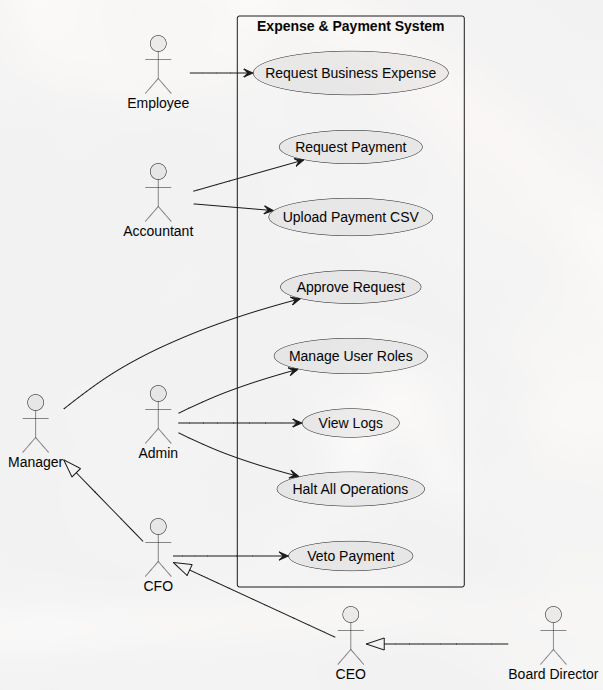
\includegraphics[width=7.18647in,height=7.17708in]{media/image0.png}\\

\subsection{User Stoeies}
\textbf{US-01:} Authentication

\begin{itemize}
\item
  \textbf{User Story:} As a registered user, I want to authenticate with
  my username and password, so that I can access features restricted to
  my specific role.
\item
  \textbf{Acceptance Criteria:}

  \begin{itemize}
  \item
    \textbf{Happy Path:}

    \begin{itemize}
    \item
      Given that I have an active account with a specific role,
    \item
      When I submit valid credentials,
    \item
      Then I am given an obfuscated token and redirected to the
      dashboard
    \end{itemize}
  \item
    \textbf{Negative path:}

    \begin{itemize}
    \item
      Given I input an invalid password, username or combination,
    \item
      When I attempt to sign in,
    \item
      Then the system rejects the request with a HTTP 401 error and
      displays ``Invalid credentials'' without revealing whether the
      username or password was wrong.
    \end{itemize}
  \item
    \textbf{Security:}

    \begin{itemize}
    \item
      Given my access token has expired,
    \item
      When I attempt to make a protected API call,
    \item
      Then the system invalidates my session and redirects me to the
      login page.
    \item
      Given 5 consecutive failed login attempts for a specific account,
    \item
      When another attempt is made within 15 minutes,
    \item
      Then the system blocks the attempt with an HTTP 429 error.
    \item
      Given a user logs out,
    \item
      When the session is destroyed,
    \item
      Then the previous token cannot be reused for subsequent requests.
    \end{itemize}
  \end{itemize}
\end{itemize}
\textbf{US-02:} Payment Upload

\begin{itemize}
\item
  \textbf{User Story:} As a user with access to uploading files, I want
  to upload a csv file, so that the file is approved and the payment
  process starts.
\item
  \textbf{Acceptance Criteria:}

  \begin{itemize}
  \item
    \textbf{Happy Path:}

    \begin{itemize}
    \item
      Given that I have an account with permission,
    \item
      When I submit a valid file,
    \item
      Then I am given a success message, and I can see its status.
    \end{itemize}
  \item
    \textbf{Negative path:}

    \begin{itemize}
    \item
      Given I input an invalid formatted csv,
    \item
      When I attempt to upload it,
    \item
      Then the system rejects the file and displays the reason.
    \end{itemize}
  \end{itemize}
\end{itemize}
\newpage
\textbf{US-03:} Business Expense Request

\begin{itemize}
\item
  \textbf{User Story:} As a user with access to business expense
  requests, I want to request a fixed sum of money and specify the reason, so that the amount
  is approved.
\item
  \textbf{Acceptance Criteria:}

  \begin{itemize}
  \item
    \textbf{Happy Path:}

    \begin{itemize}
    \item
      Given that I have an account with permission,
    \item
      When I submit an expense request,
    \item
      Then I am given a success message, and I can see its status.
    \end{itemize}
  \item
    \textbf{Negative path:}

    \begin{itemize}
    \item
      Given I input an invalid amount,
    \item
      When I attempt to request it,
    \item
      Then the system rejects the sum and displays the reason.
    \item
      Given I input too many requests in less than 1 hour,
    \item
      When I attempt to request it,
    \item
      Then the system rejects the request and displays the reason.
    \end{itemize}
  \end{itemize}
\end{itemize}
\textbf{US-04:} Request Status Checking

\begin{itemize}
\item
  \textbf{User Story:} As a user with a request, I want to check the
  status, so that I know my situation.
\item
  \textbf{Acceptance Criteria:}

  \begin{itemize}
  \item
    \textbf{Happy Path:}

    \begin{itemize}
    \item
      Given that I have an account with a request,
    \item
      When I look at a pending request,
    \item
      Then I can see who still needs to approve it.
    \item
      Given that I have an account with a denied,
    \item
      When I look at the denied request,
    \item
      Then I can see who denied it and if they left any comments.
    \item
      Given that I have an account with an approved request,
    \item
      When I look at the request,
    \item
      Then I can see it added to my requests history.
    \end{itemize}
  \end{itemize}
\end{itemize}
\textbf{US-05:} Request Management

\begin{itemize}
\item
  \textbf{User Story:} As a user with requests that need to be approved
  or denied, I want to decide, so that the payments proceed.
\item
  \textbf{Acceptance Criteria:}

  \begin{itemize}
  \item
    \textbf{Happy Path:}

    \begin{itemize}
    \item
      Given that I have an account with a request that needs approval,
    \item
      When I look at the pending request,
    \item
      Then I can press either approve or deny button.
    \item
      Given that I have an account that is not CEO, CFO, Board Director,
    \item
      When I look at the request,
    \item
      Then I can press a button to forward the request to a higher-up.
    \item
      Given that I have an account with a request that has a file
      attached,
    \item
      When I look at the request,
    \item
      Then I can download the file to my computer.
    \item
      Given that I have an account with a request that has a file
      attached,
    \item
      When I took actions related to the request,
    \item
      Then I can leave a comment/reason for my actions.
    \end{itemize}
  \end{itemize}
\end{itemize}
\textbf{US-06:} Veto Request

\begin{itemize}
\item
  \textbf{User Story:} As a user with access to the veto function, I
  want to veto a payment, so that the payments are stopped.
\item
  \textbf{Acceptance Criteria:}

  \begin{itemize}
  \item
    \textbf{Happy Path:}

    \begin{itemize}
    \item
      Given that I have an account with veto access that needs approval,
    \item
      When I look at the pending or approved, but not started, request,
    \item
      Then I can press the veto button to cancel immediately.
    \end{itemize}
  \end{itemize}
\end{itemize}
\textbf{US-07:} System Admin

\begin{itemize}
\item
  \textbf{User Story:} As a user with a system admin role, I want to
  read logs, manage users' roles and have the option to halt all
  transactions, so that other users can do their jobs and any fraud
  attempt can be stopped.
\item
  \textbf{Acceptance Criteria:}

  \begin{itemize}
  \item
    \textbf{Happy Path:}

    \begin{itemize}
    \item
      Given that I have an account with system admin access,
    \item
      When I look at the designated logs tab,
    \item
      Then I can see all transactions and logs.
    \item
      Given that I have an account with system admin access,
    \item
      When I look at the \emph{users} tab,
    \item
      Then I can see all the users and modify their roles.
    \item
      Given that I have an account with system admin access,
    \item
      When I see a transaction fraud or security breach,
    \item
      Then I can press the halt all transactions button.
    \end{itemize}
  \end{itemize}
\end{itemize}

\section{Business Process \& Workflow}

\subsection{Payment Requests}
\subsubsection{\textit{Process Diagram}}

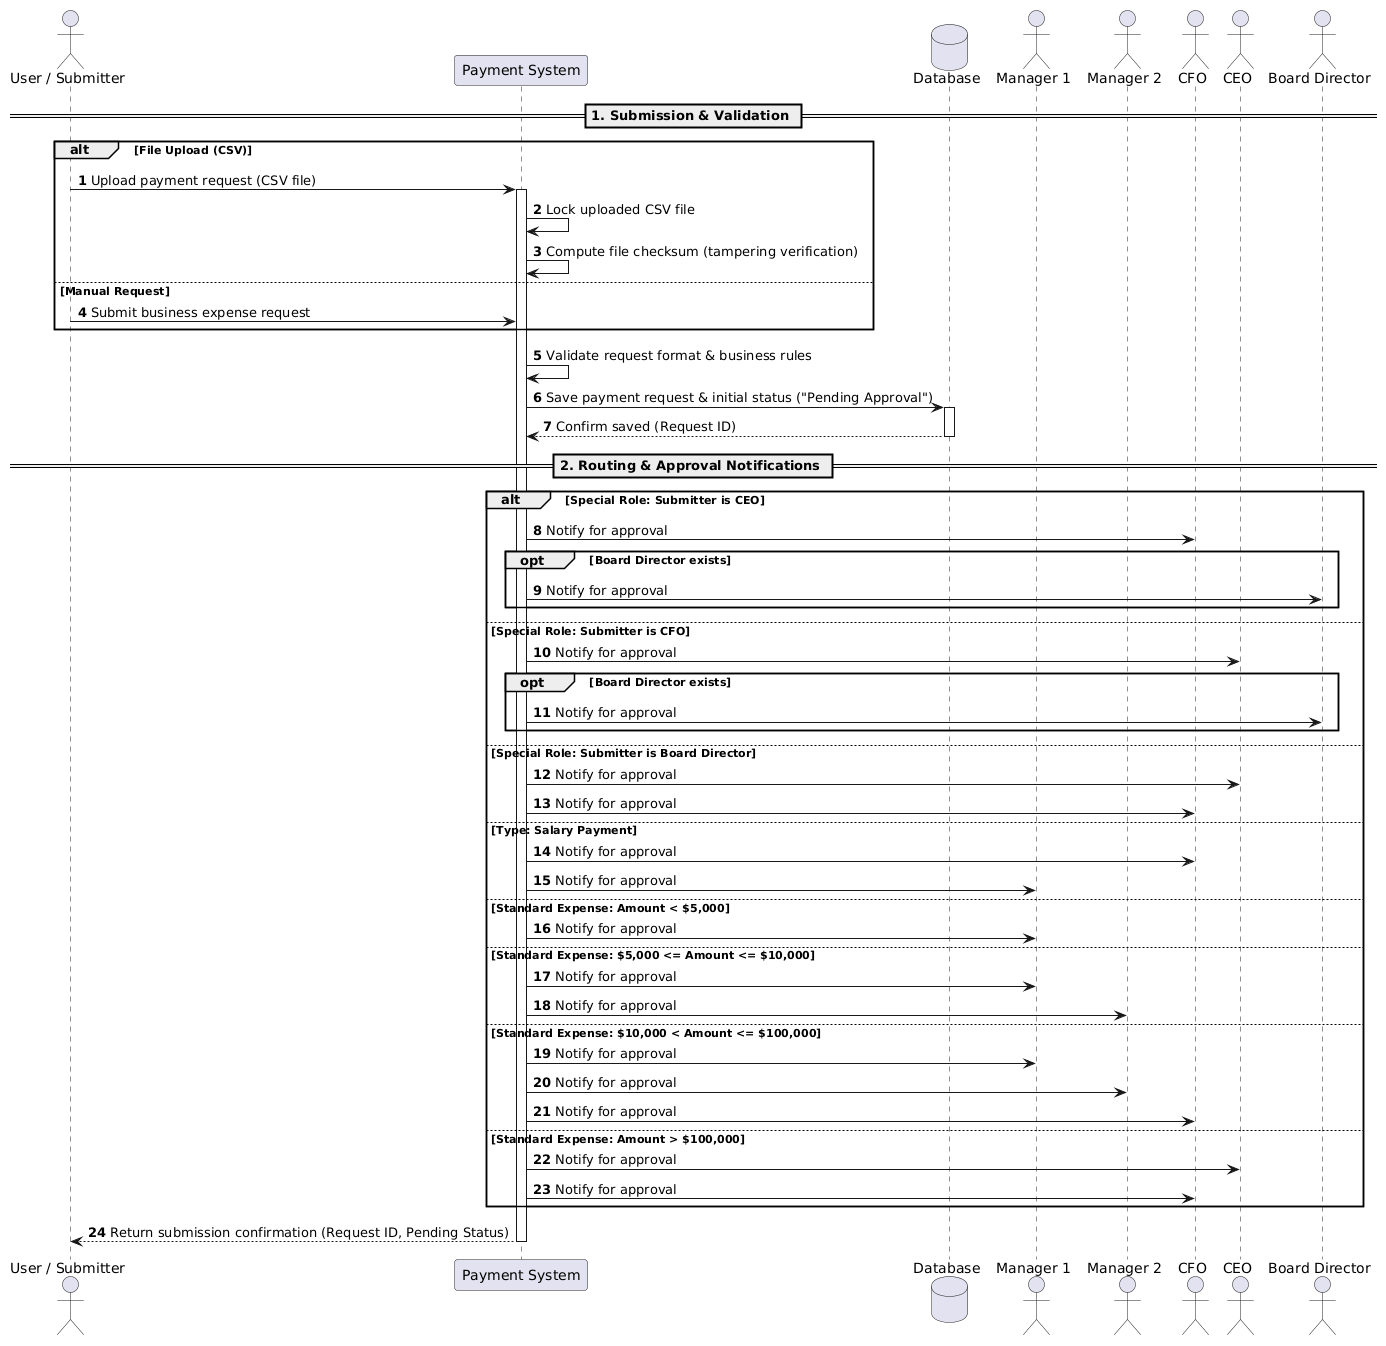
\includegraphics[width=7.18647in,height=7.17708in]{media/image1.png}

\subsubsection{\textit{Workflow Narrative}}

\begin{enumerate}
\def\labelenumi{\arabic{enumi}.}
\item
  The user uploads a csv file or requests a business expense.
\item
  The system validates the request, adds it to the database, and
  notifies the parties for approval.
\end{enumerate}

\subsubsection{\textit{Business Rules \& Constrains}}

\begin{itemize}
\item
  A request of less than \$5000 will require 1 manager's approvement.
\item
  A request of more than \$5000 will require 2 managers' approvement.
\item
  A request of more than \$10,000 will require 2 managers and the CFO's
  approvement.
\item
  A request of more than \$100,000 will require the CEO's and CFO's
  approvement.
\item
  Should a request come from the CEO, then the request will need CFO's
  and, if any, a board director's approval. Similarly, if the request
  comes from the CFO, then the CEO's and, if any, a board director's
  approval. Finally, should the request come from a board director, then
  it requires the CEO's and CFO's approval.
\item
  All salary approvals will require CFO's and Manager's approval.
\item
  When a csv file is uploaded, the system locks the file and computes
  the checksum for tampering verification.
\end{itemize}

\subsection{Payment Signature}

\subsubsection{\textit{Process Diagram}}

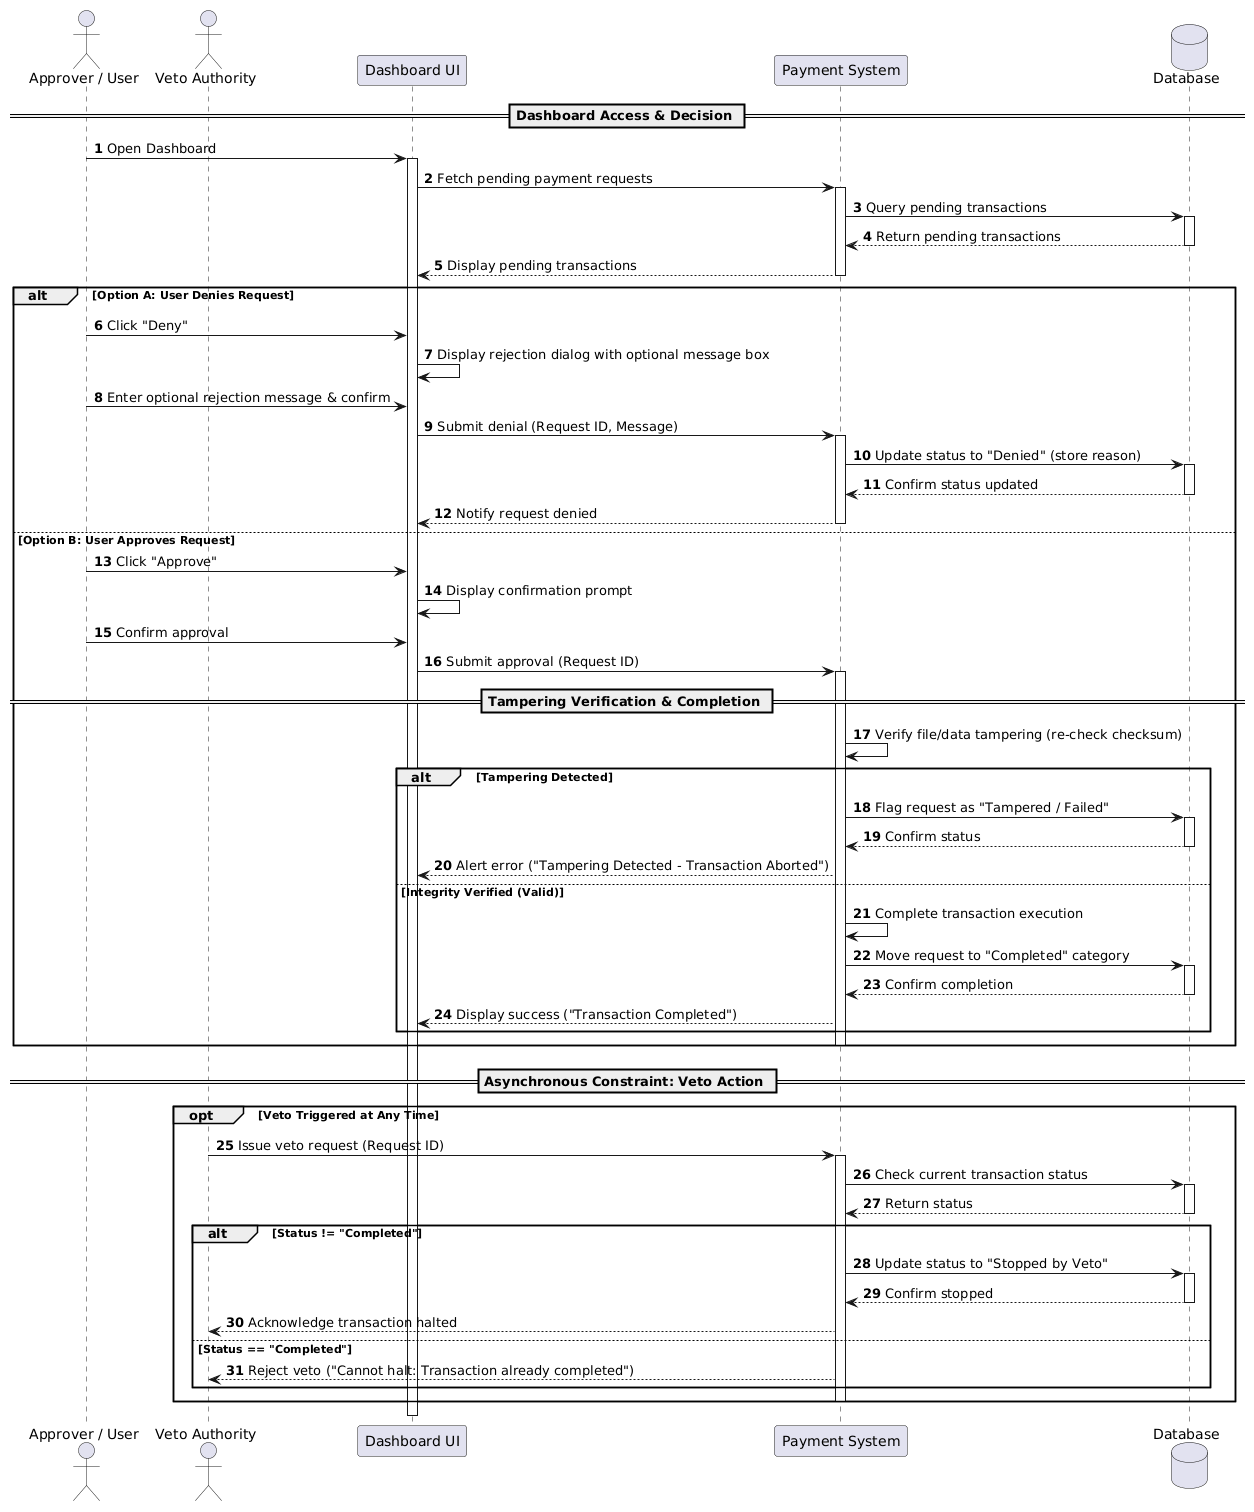
\includegraphics[width=6.56976in,height=7.91415in]{media/image2.png}

\newpage
\subsubsection{\textit{Workflow Narrative}}

\begin{enumerate}
\def\labelenumi{\arabic{enumi}.}
\item
  User opens the dashboard and clicks on either the approve or deny
  button.
\item
  A confirmation box will appear.
\item
  Should the user deny the request, a box with the option to leave a
  message will appear.
\end{enumerate}

\subsubsection{\textit{Business Rules \& Constrains}}

\begin{itemize}
\item
  If a transaction is approved, the system automatically checks
  tampering and completes the transaction.
\item
  The request is moved to the completed category.
\item
  A veto request can stop the transaction at any time, unless already
  completed.
\end{itemize}
\newpage
\section{Business Solution Architecture \& System Design}

\subsection{High-Level Architecture Overview}

\textbf{Architectural Style:} Decoupled Single-Page Application with a
REST API. \\
\textbf{Frontend:} Vue. \\ 
\textbf{Backend:} Spring Boot - kotlin. \\
\textbf{Database}: PostgreSQL Relational. \\
\textbf{Auth \& Security:} Obfuscated tokens, Argon2 hashing, CORS and
Redis. \\
\textbf{C6 component diagram, that can also be found
\href{https:////www.plantuml.com/plantuml/png/bLVVSzis4dxNNx7nWq-PiKypDtdAtDr4bjNMgLqhbXC_Qa1oHQC60HO0PQkT_k_T1GWRD1qdUIC1xBS_kFY-vGVdXVLTeoPlf2vLLo7yT_5kjdYtMPYcDHgr__zaugLN28yhS2f5RKNp7auxeU36sBkjClTmB_qjpDjMoL9uQJJCkqhwsSty70xXtDGmhskBTTYRJ5PedT5JR5fbzeX7SB3i7s5wXNzqw3pQjmUqlkwAHde7HUUaHkS07rhK3i76OmTl4vWeIzDfBxGdi_dZ2qm_4xAeUhpumdZg3fnGmkvXiVu2MwdGFO4rGeiQBHbSn2UOmM9v2LDAqPfT3tQ5EudtxWX4NAKdOs67tg03wR5XnCd2K20Kl9swLd1AKjSAZrS4crUC0Rzq-E_VNO0sTAGG3YluVCOewxqZmCtomK-Tjx95Hk870bcTiSbAx1l-GbHal1Txk1MwKkGBMh4tdQTOSX1bwfesDouiaVc2RArGyazoUHutuH3MPyiB1b-U_qebE1LULARcOYZJLJV2bxUykp1AOUaTYAm3o0ENfYpvin5qYVogAt1OTbRwFGY5rWzhT5fCBLRISNPanpY7S6tkKCFQ6uknx7I07-Qbbpi45m-IZGy72oNAEoKTDO8L7a79HhARWPUg24Wgn2fKI8th7IffdAyjhZ-Tyrlmww1pQCb5mJbp9h5vKX_6rFXxegwEBxNQPpU0AojncEZcX1gq8eIfQEMcw5_ONMkvz2V6U3YXH91XLzG3yDS409wkuZJLSKFDwz6oRQhiJs7bu0akxHp1ul9gVGHpMnlzdz1pGibAU7InUfH8R7xNdxJeZDhr1G1PaMV2eLo6mOZEtsvARnL_5te6pjGQfM8OLylrzRCbQZAfqpUJpdL2bzJLfSNWGoZOePNRlfrwXy-yKcipO7AyYgzKDrz-HmHBNRL6QkzWQsoa1EO2qw8DFjqeo_ZHD_JHaykJH4pBI4m_wbNgIkvanMGwxAYnyyWoGZsMkN-7G_Y2tloePnlOwmWIREnWPY_o_BpEHibolwaxOIl6Ffalc1pCAQp23lpCEo_q6ynWVhcApibfYGue7dJ1ruMuGtkyk4NgSliU2cNAEmSErVOu1GLzrcZXpVz0QkcbyCQ-VRaTIhVRjCAwS1duKvxHZlKKZTt94lFuqaf-0JYcOEuoJNYb1Lm4OTIm256xljiV9j539MjPICK5uo0gAxP-s0YZNEzxwTsWhgNc84wbAphha5NWIPcNlFsLK1R6s4fg3YOIswpt2SxJ8hEsTZAx2gCWXCgg41YF-kAoyuLv0AA-roiHsTA1R9hEYqBXs6qe1vzw4ZAGsYCtSO7KKGZuuD5geUW1o-vLhk3APF7s-hcAiA-6kWpOw9AOGjHcew4qUYjjWzKHFJQDz1uhJZr5Qx6a8e_xo69hDahiGw-o-i0yIkKvhsLHXBsFgpalNVJKNFLg1O6DPUpTw1MjaywZBf5S_ZsP_0kMgK1SE2lAKDW9QLysWBbMPDDMtmNiyPVhwzMQaEXuDc8bWpHEqNLvTZYDKEbaFpWvc0MoGfUV3mRXt4kQnYr22WYbKCh5IPFL9Yh74muXVrnV_jQx7m6biIBGJIzsiEExIATwmbnzpJXNjol3ZH13mCIeNpDC0ZMmZLBJXTfz6sAaEGbbD1D_4sge80ceLu9Psirng7zINvPHImBoCArS7GO4butXpFefh3oXL-tJNq4-TZ12biV8FbEQ5Tf6njaG3k558KdDDuGOw4X0yL4IU57gcgp6HcDXo8mJhvOMqpWpHXXHUZ9FiSzOdKSacNB8env3fRlDlHV9lezX7FShvjcyadAAJSBSCqlCpwO1UuGp58mRApswFg7oLkWQuN18ytsG0xi1THAZfXBnw6ruz4v3TxZN7qzF5Y-XZFNWsigwHkiU9IM54a35bXOPkkVvLFQC6mQ1VUhGIdJPG9lkvQWg0xjLP707bMc4rA4wdUlBao1oY_vNHbHChlUnfFRfpuQr0Wuvy5GDEaR_DYd-KHtY_-LOz6BBRT7cbCjZPko0ou8HH1nZ60H5mmus_1Sp-jzy_jSJZbEMwVy8o23SsaW-k6F9xtyR2WBa7FQE3l64MST6-O2wwXhr3m00}{here:}}

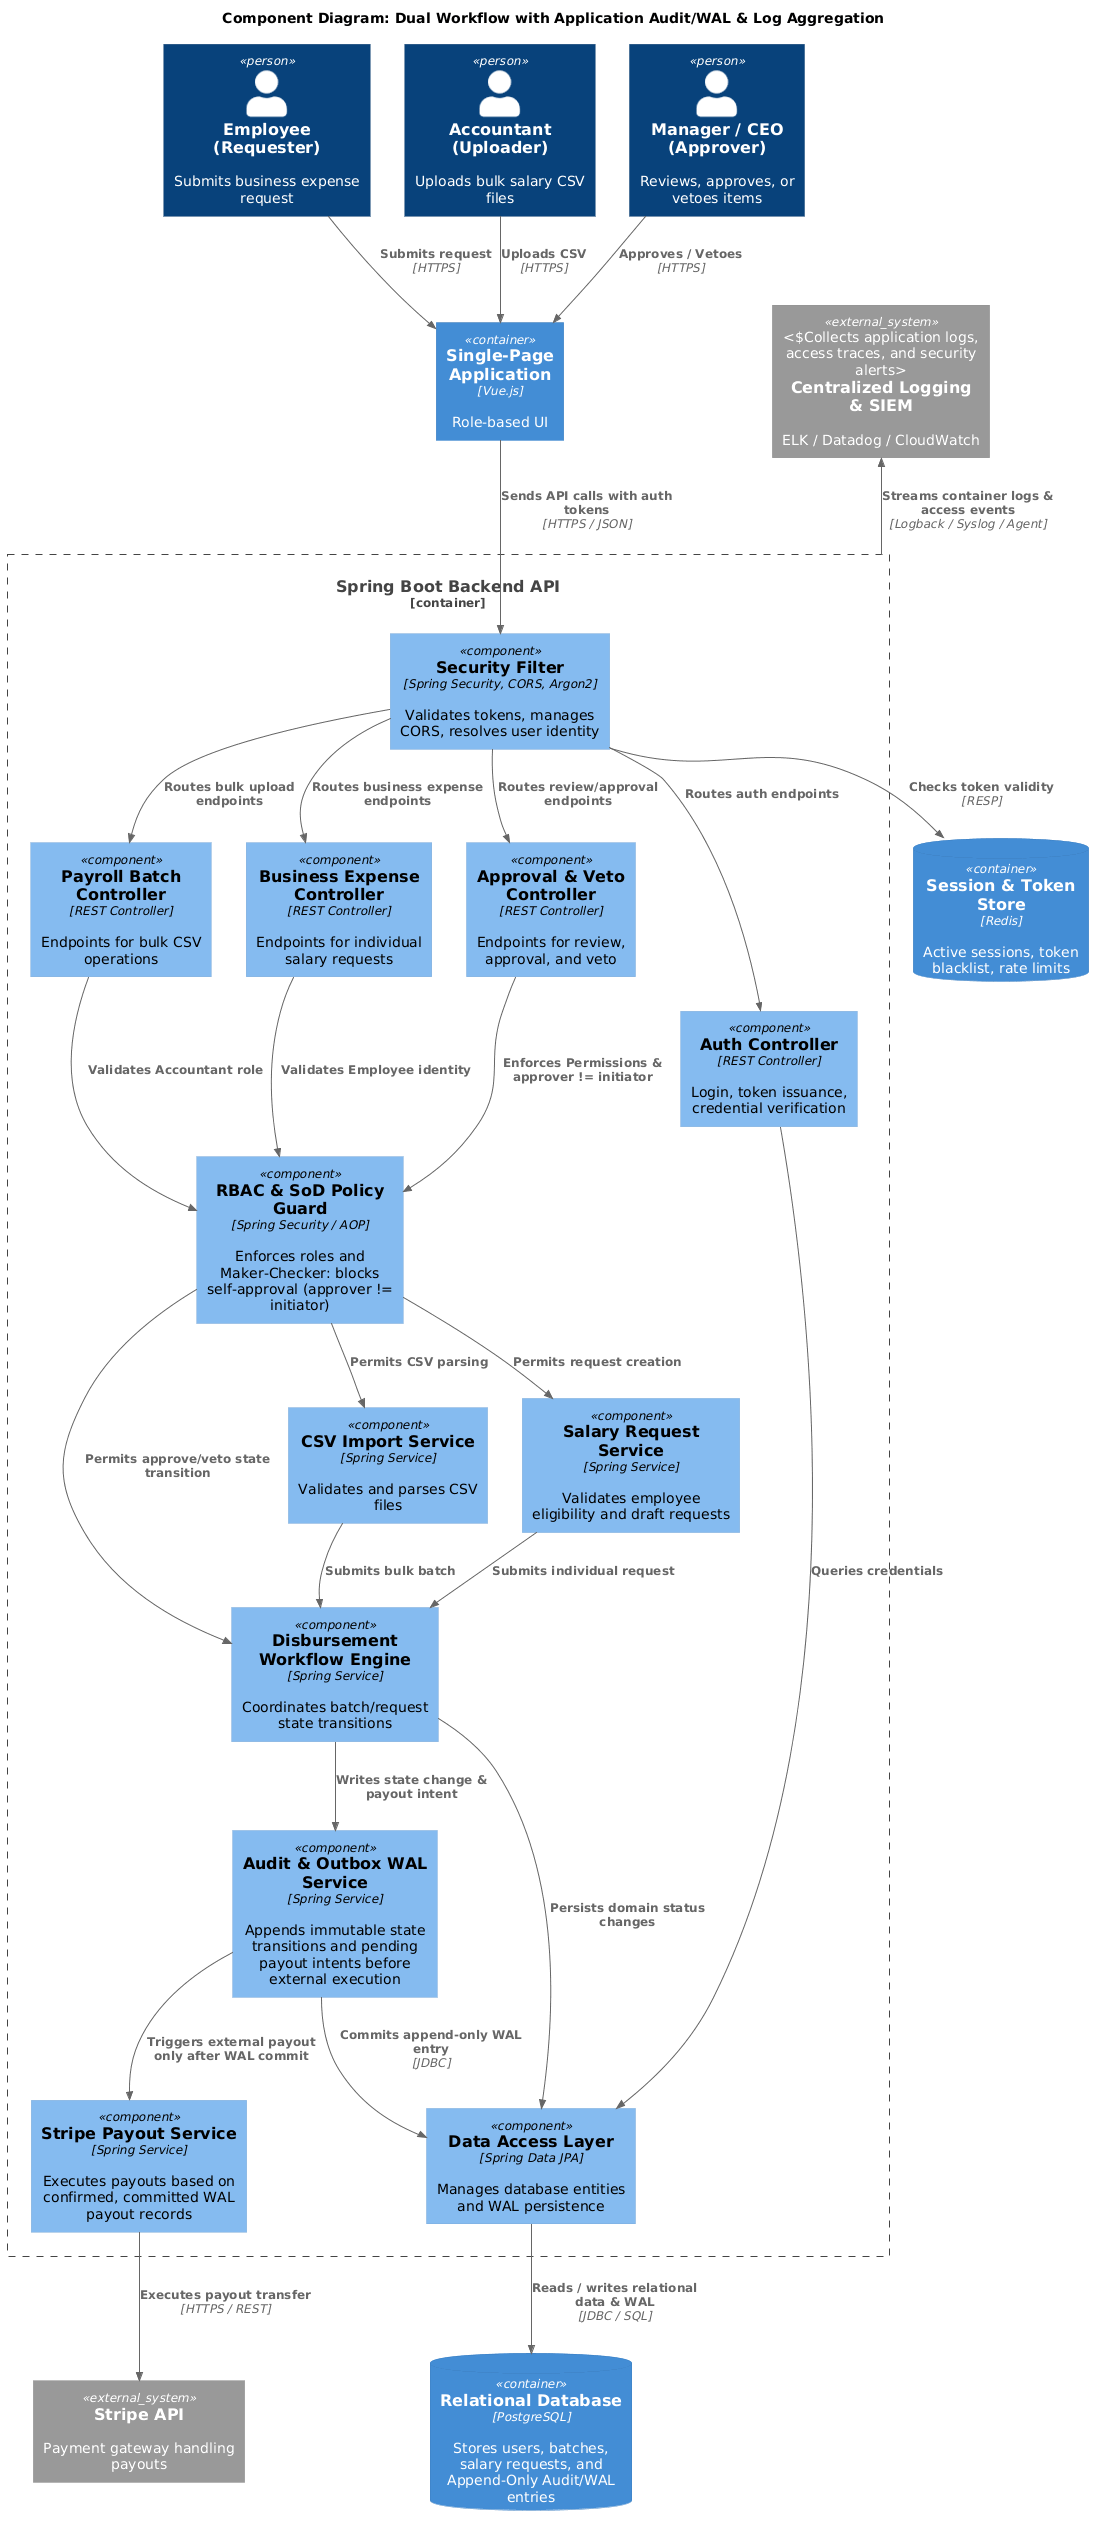
\includegraphics[width=5.89497in,height=9.32986in]{media/image3.png}
\subsection{Data Model \& Database Schema}

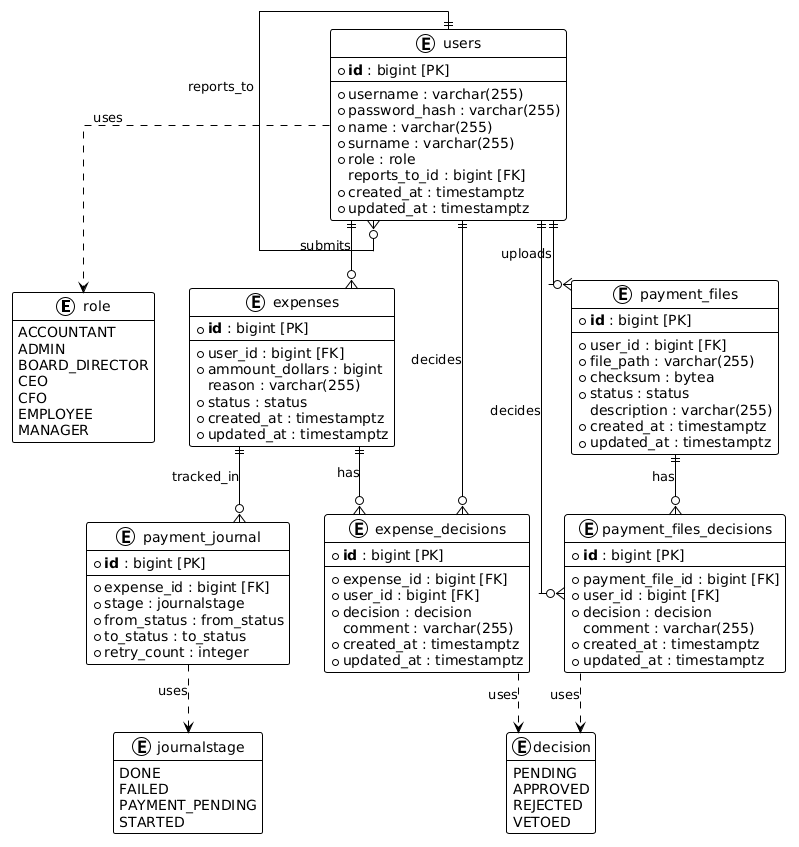
\includegraphics[width=7.35993in,height=6.65224in]{media/image4.png}

\subsection{Security, Authentication \& Authorization Architecture}

\textbf{Authentication Flow:} The id of a user is obfuscated to a UUID.
Redis cache translates between the two.\\
\textbf{Token Strategy:} Short-lived obfuscated token. \\
\textbf{Role-Based Access Control:}\\
All authentication endpoints under \texttt{/api/v1/auth/*} (such as login and token issuance) are publicly accessible without authentication. Once an identity is verified, access to protected endpoints is strictly governed by the roles outlined in:
\begin{longtable}[]{@{}
  >{\centering\arraybackslash}p{(\linewidth - 4\tabcolsep) * \real{0.3333}}
  >{\raggedright\arraybackslash}p{(\linewidth - 4\tabcolsep) * \real{0.3333}}
  >{\raggedright\arraybackslash}p{(\linewidth - 4\tabcolsep) * \real{0.3333}}@{}}
\toprule\noalign{}
\begin{minipage}[b]{\linewidth}\centering
Role
\end{minipage} & \begin{minipage}[b]{\linewidth}\raggedright
Accessible Routes
\end{minipage} & \begin{minipage}[b]{\linewidth}\raggedright
Permissions
\end{minipage} \\
\midrule\noalign{}
\endhead
\bottomrule\noalign{}
\endlastfoot
System Admin & /api/v1/requests/expenses/*, /api/v1/admin/*, /api/v1/user/*
/api/v1/logs/* & Can manage roles and see obfuscated logs (sensitive
information is redacted) \\
Employee & /api/v1/requests/expenses/* & Can only see/post own request \\
Manager & 

/api/v1/requests/* & Can see own requests and
subordinates\textquotesingle{} requests or csv files and approve/co-approve any of them \\
Board Director/CEO/CFO & /api/v1/requests/*
& Can see every request or payment, can approve/co-approve or delete
them \\
Accountant & /api/v1/requests/* & Can see its own requests and upload payments \\
\end{longtable}

\section{API Contracts \& Endpoint Specifications}

\subsection{Authentication Endpoint}

\emph{POST /api/v1/auth/login} \\
\textbf{Auth:} Public \\
\textbf{Request Body:} \\
\begin{lstlisting}[language=json]
{
  "username" : "usernameExample",
  "password" : "passwordExample"
}
\end{lstlisting}
\textbf{Response 200 OK}

\begin{lstlisting}[language=json]
{
  "token": "eyJhbGciOiJIUzI1NiIsInR5cCI6IkpXVCJ9...",
  "role": "employee",
  "name": "Name1"
}
\end{lstlisting}
\textbf{Error Response 401 Unauthorized}
\begin{lstlisting}[language=json]
{
  "error": "AUTH_FAILED", 
  "message": "Invalid email or password"
}
\end{lstlisting}

\subsection{Request Business Expense}

\emph{POST /api/v1/requests/request/upload} \\
\textbf{Auth:} Token, Role: All \\
\textbf{Request Body:} \\
\begin{lstlisting}[language=json]
{
  "token" : "eyJhbGciOiJIUzI1NiIsInR5cCI6IkpXVCJ9...",
  "ammountUsd" : "100",
  "reason" : "Businness Meal with business partnenerr"
}
\end{lstlisting}
\textbf{Response 200 OK}

\begin{lstlisting}[language=json]
{

  "id": 9007199254740991,
  "reason": "string",
  "createdAt": "2026-11-28T12:14:35.189Z",
  "updatedAt": "2026-11-28T12:14:35.189Z",
  "status": "PENDING",
  "ammountOfDollars": 9007199254740991,
  "needsApprovalBy": [
    "string"
  ],
  "approvedBy": [
    "string"
  ],
  "rejectedBy": [
    "string"
  ]

}
\end{lstlisting}

\subsection{Upload Payment File}

\emph{POST /api/v1/requests/payments/upload} \\
\textbf{Auth:} Token, Role = "Manager, CEO, CFO, Board Director, Accountant" \\
\textbf{Request Body:} \\
\begin{lstlisting}[language=json]
{
  "token" : "eyJhbGciOiJIUzI1NiIsInR5cCI6IkpXVCJ9...",
  "file" : "file.csv",
  "reason": "Any reason"
}
\end{lstlisting}
\textbf{Response 200 OK}

\begin{lstlisting}[language=json]
{
  "id": 9007199254740991,
  "reason": "string",
  "createdAt": "2026-11-28T12:15:27.083Z",
  "updatedAt": "2026-11-28T12:15:27.083Z",
  "status": "PENDING",
  "needsApprovalBy": [
    "string"
  ],
  "approvedBy": [
    "string"
  ],
  "rejectedBy": [
    "string"
  ]
}
\end{lstlisting}

\textbf{Error Response 500 Bad Request}
\begin{lstlisting}[language=json]
{
  "error": "Malformed CSV", 
  "message": "Error on row X col Y, because Z"
}
\end{lstlisting}


\subsection{Reading Requests}

\emph{GET /api/v1/requests/payments/personal} \\
\textbf{Auth:} Token, Role = "Manager, CEO, CFO, Board Director, Accountant" \\
\textbf{Request Body:} \\
\begin{lstlisting}[language=json]
{
  "token" : "eyJhbGciOiJIUzI1NiIsInR5cCI6IkpXVCJ9..."
}
\end{lstlisting}
\textbf{Response 200 OK}

\begin{lstlisting}[language=json]
{
  [
  {
    "id": 9007199254740991,
    "reason": "string",
    "createdAt": "2026-11-28T12:24:57.132Z",
    "updatedAt": "2026-11-28T12:24:57.132Z",
    "status": "PENDING",
    "needsApprovalBy": [
      "string"s
    ],
    "approvedBy": [
      "string"
    ],
    "rejectedBy": [
      "string"
    ]
  }
]
}
\end{lstlisting}

\subsection{Additional responses if not specified}
\textbf{Error Response 401 Unauthorized}
\begin{lstlisting}[language=json]
{
  "error": "REQUEST_FAILED", 
  "message": "You cannot do that"
}
\end{lstlisting}

\textbf{Error Response 500 Internal Server Error}
\begin{lstlisting}[language=json]
{
  "error": "Server down"
}
\end{lstlisting}


\textbf{Error Response 503 Service Unavailable}
\begin{lstlisting}[language=json]
{
  "error": "Server down for maintenance", 
  "message": "Expected to be up in HH:MM"
}
\end{lstlisting}

\section{UI/UX}

\subsection{Screenflow}

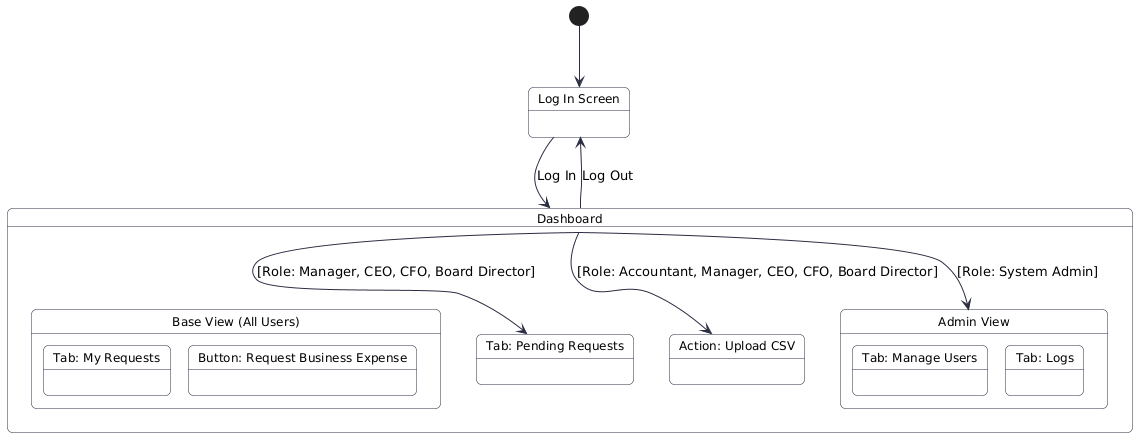
\includegraphics[width=\linewidth, keepaspectratio]{media/image5.png}

\subsection{Wireframes}

\subsubsection{Logging in}
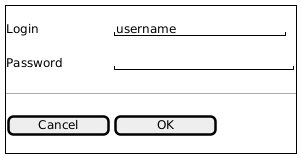
\includegraphics{media/LogIn.png}
\subsubsection{Employee}
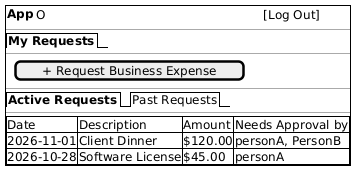
\includegraphics{media/ActiveRequests.png} \\
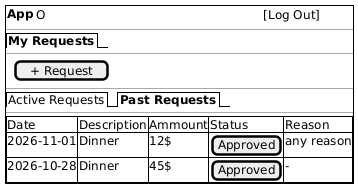
\includegraphics{media/PastRequests.png}
\subsubsection{Accountant}
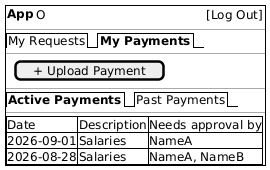
\includegraphics{media/ActivePayments.png} \\
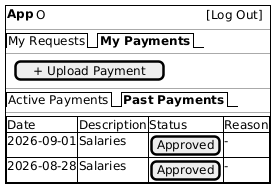
\includegraphics{media/PastPayments.png}
\subsubsection{Manager/CEO/CFO/Board Director}
\begin{figure}[htbp]
    \centering
    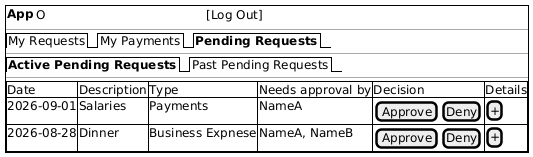
\includegraphics[width=\linewidth, keepaspectratio]{media/PendingRequests.png}
\end{figure}
\begin{figure}[htbp]
    \centering
    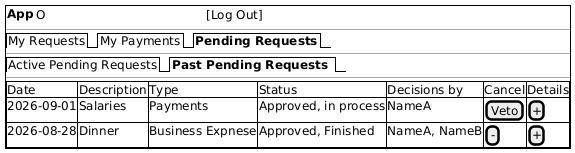
\includegraphics[width=\linewidth, keepaspectratio]{media/PastPendingRequests.png}
\end{figure}


\subsubsection{Admin}
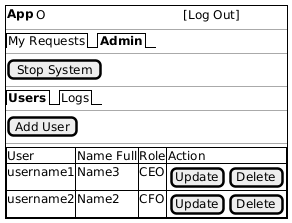
\includegraphics{media/UserManagement2.png} \\
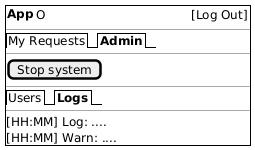
\includegraphics{media/Logs.png}
\end{document}